% id: 79-e2
% book: 100발100중 3-2 기말 · 01 3-2 기말(원의 성질·통계·부록)
% section: 서술형 문제
% figure: crop:fig-79-e2-2.png
% answer: $72.5$점
% answer_source: 예제 모범답안
% variant_level: 0 (원본 전사)
% 이 파일은 build.mjs 가 items.json 에서 만든다. 고칠 때는 items.json 을 고친다.
\smash{\raisebox{1.5mm}{\dmkichul{100발100중 3-2 기말 79쪽 예제 2 · 예제}}}
\noindent\begin{minipage}[t]{0.58\linewidth}\vspace{0pt}\raggedright 그림은 민지네 반 학생 15명의 중간고사와 기말고사의 수학 성적을 조사하여 나타낸 산점도이다. 이때 중간고사에 비하여 기말고사 수학 성적이 올라간 학생들의 중간고사 수학 성적의 평균을 구하고, 그 과정을 서술하시오. \mbox{[6점]}\end{minipage}\hfill\begin{minipage}[t]{0.4\linewidth}\vspace{0pt}\centering 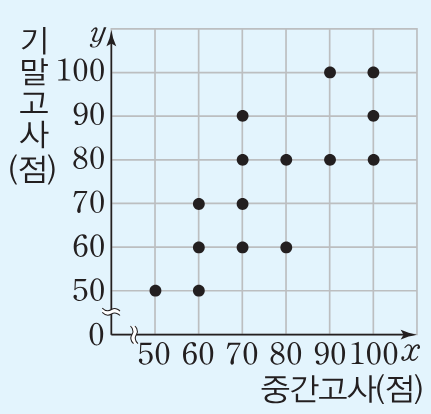
\includegraphics[width=103.3pt]{figures/fig-79-e2-2.png}\end{minipage}\par
